%%
% This is an Overleaf template for presentations
% using the TUM Corporate Desing https://www.tum.de/cd
%
% For further details on how to use the template, take a look at our
% GitLab repository and browse through our test documents
% https://gitlab.lrz.de/latex4ei/tum-templates.
%
% The tumbeamer class is based on the beamer class.
% If you need further customization please consult the beamer class guide
% https://ctan.org/pkg/beamer.
% Additional class options are passed down to the base class.
%
% If you encounter any bugs or undesired behaviour, please raise an issue
% in our GitLab repository
% https://gitlab.lrz.de/latex4ei/tum-templates/issues
% and provide a description and minimal working example of your problem.
%%

\PassOptionsToClass{onlytextwidth}{beamer}

\documentclass[
  german,            % define the document language (english, german)
  aspectratio=169,    % define the aspect ratio (169, 43)
  % handout=2on1,       % create handout with multiple slides (2on1, 4on1)
  % partpage=false,     % insert page at beginning of parts (true, false)
  % sectionpage=true,   % insert page at beginning of sections (true, false)
]{tumbeamer}


% load additional packages
\usepackage{tikz}
\usepackage{circuitikz}
\usepackage{url}
\usepackage{hyperref}
\usepackage{pgf}
\usepackage{pgfplots}
\usepackage{babel}[ngerman]
\usepackage{csquotes}[autostyle]
\usepackage[useregional]{datetime2}
\usepackage{float}
\usepackage{graphicx}
\usepackage{amsmath}
\usepackage{amssymb}
%\usepackage{xcolor}
\usepackage[cache=true]{minted}
\usemintedstyle{borland}
%\usepackage{listings}
%\usepackage{tikz-timing}
%\usepackage{ifthen}
\usepackage{ulem}
\usepackage{enumerate}
\usepackage{karnaugh-map}
%\usepackage{forest}


% tikz
\usetikzlibrary{overlay-beamer-styles}
\usetikzlibrary{arrows,backgrounds,positioning,shapes,patterns,patterns.meta,matrix,arrows.meta,shapes.geometric}
\usetikzlibrary{matrix, fit, calc}
%\usetikzlibrary{automata}

% requires circuitikz >= 1.1.0
% for distros with older distributions, install TeX Live manually
% instead of using your package manager
% see: https://tug.org/texlive/quickinstall.html
\ctikzset{logic ports=ieee}

% minted
\setminted{
    fontsize=\small, 
    frame=none,
    breaklines=false,
}

% lstlisting
% \lstset{escapeinside={<@}{@>}}

% image path
\graphicspath{ {./resources/} }

% commands
\newcommand{\n}[1]{\overline{#1}}

% https://tex.stackexchange.com/a/7045
\newcommand*\circled[1]{\tikz[baseline=(char.base)]{
		\node[shape=circle,draw,inner sep=2pt, font=\scriptsize] (char) {#1};}}
	
\newcommand*\colorcirc[1]{\tikz[baseline=(char.base)]{
			\node[shape=circle,fill=#1,inner sep=2pt] {};}}

% beamer
\setbeamercolor{footnote}{fg=black}
\setbeamercolor{footnote mark}{fg=black}

% presentation metadata
\title{Übung 13: SAT und Physical \\Design}
\subtitle{Einführung in die Rechnerarchitektur}
\author{Niklas Ladurner}

\institute{\theChairName\\\theDepartmentName\\\theUniversityName}
\date{\DTMdisplaydate{2025}{01}{24}{-1}}

\footline{\insertauthor~|~\insertshorttitle~|~\insertshortdate}


% macro to configure the style of the presentation
\TUMbeamersetup{
  title page = TUM tower,         % style of the title page
  part page = TUM toc,            % style of part pages
  section page = TUM toc,         % style of section pages
  content page = TUM more space,  % style of normal content pages
  tower scale = 1.0,              % scaling factor of TUM tower (if used)
  headline = TUM threeliner,      % which variation of headline to use
  footline = TUM default,         % which variation of footline to use
  % configure on which pages headlines and footlines should be printed
  headline on = {title page},
  footline on = {every page, title page=false},
}

\setbeamercolor{enumerate item}{fg=black}

\begin{document}

\maketitle

\begin{frame}[c, fragile]{}{}
	\begin{center}
		\LARGE  Keine Garantie für die Richtigkeit der Tutorfolien.

		\Large Bei Unklarheiten/Unstimmigkeiten haben VL/ZÜ-Folien recht!
	\end{center}
\end{frame}

\begin{frame}[c]{SAT}{}
	\begin{itemize}
		\item Satisfiability $\rightarrow$ Erfüllbarkeit einer boolschen Funktion feststellen
		\item moderne Solver können sichere Aussage über SAT/UNSAT treffen, ohne alle Variablenbelegungen durchzuprobieren $\rightarrow$ einigermaßen effizient lösbar\footnote{SAT ist und bleibt aber trotzdem NP-vollständig :)}
		\item DPLL und Konfliktgraphen nicht mehr relevant für ERA
		\item Formulierung als KNF (Konjunktive Normalform, CNF): OR in den Klammern, AND dazwischen, z.B.:\[
			      (x_1+x_2+x_3)\cdot(\n{x}_2+x_4+x_5)\cdot(\n{x}_1+x_3+\n{x}_5)\]
	\end{itemize}
\end{frame}

\begin{frame}[c, fragile]{SAT: Schaltkreisäquivalenz}{}
	\begin{columns}[c]
		\begin{column}{0.5\textwidth}
			\begin{center}
				\begin{circuitikz}
					\tikzset{
						bbox/.style = {shape=rectangle, dashed, draw=blue, inner xsep=8pt, inner ysep=15pt},
						blabel/.style={inner sep=0, anchor=north west, font=\tiny, color=blue, yshift=-2}
					}
					\def\spacing{0.5cm}

					\node[nand port] (nand) at (-2,0) {};
					\draw (nand.in 1) -- ++(-\spacing, 0) node (a1)  {} node[left] {$a$};
					\draw (nand.in 2) -- ++(-\spacing, 0) node (b1) {} node[left] {$b$};
					\draw (nand.out) -- ++(\spacing, 0) node (c) {} node[right] {$c$};

					\node[or port] at (-2, -6*\spacing) (or) {};
					\draw (or.in 1) -- ++(-\spacing, 0) node (a2) {} node[left] {$a$};
					\draw (or.in 2) -- ++(-\spacing, 0) node (b2) {} node[left] {$b$};
					\draw (or.out) -- ++(\spacing, 0) node (d) {} node[right] {$d$};
					\node at (or.bin 1) [notcirc, left]{};
					\node at (or.bin 2) [notcirc, left]{};

					\node[bbox, fit=(a1) (nand)] (rect1) {};
					\node[blabel] at (rect1.south west) {Schaltkreis 1};
					\node[bbox, fit=(a2) (or)] (rect2) {};
					\node[blabel] at (rect2.south west) {Schaltkreis 2};

					\node[xor port] at (-2+2.5*\spacing, -3*\spacing) (xor) {};
					\draw (xor.out) -- ++(0.5*\spacing, 0) node (e) {} node[right] {$e$};
					\draw (nand.out) -- ++(\spacing, 0) |- (xor.in 1) -- (xor.in 1);
					\draw (or.out) -- ++(\spacing, 0) |- (xor.in 2) -- (xor.in 2);
				\end{circuitikz}
			\end{center}
		\end{column}
		\begin{column}{0.5\textwidth}
			\[
				\begin{array}{|c|c|c|}
					\hline
					c & d & e = c \oplus d \\
					\hline
					0 & 0 & 0              \\
					0 & 1 & 1              \\
					1 & 0 & 1              \\
					1 & 1 & 0              \\
					\hline
				\end{array}
			\]
			\begin{itemize}
				\item existiert eine Belegung von $a, b$, sodass $e=1$, dann sind die beiden Schaltkreise für diese Belegung nicht äquivalent
				\item eine solche Schaltung heißt Miter
				\item KNF kann durch Tseitin-Transformation aufgestellt werden
			\end{itemize}
		\end{column}
	\end{columns}

\end{frame}

\begin{frame}[c, fragile]{Einschub: Tseitin-Transformation}{}
	\begin{columns}[c]
		\begin{column}{0.5\textwidth}
			\begin{center}
				\begin{circuitikz}
					\tikzset{
						bbox/.style = {shape=rectangle, dashed, draw=blue, inner xsep=8pt, inner ysep=15pt},
						blabel/.style={inner sep=0, anchor=north west, font=\tiny, color=blue, yshift=-2}
					}
					\def\spacing{0.5cm}

					\node[nand port] (nand) at (-2,0) {};
					\draw (nand.in 1) -- ++(-\spacing, 0) node (a1)  {} node[left] {$a$};
					\draw (nand.in 2) -- ++(-\spacing, 0) node (b1) {} node[left] {$b$};
					\draw (nand.out) -- ++(\spacing, 0) node (c) {} node[right] {$c$};

					\node[or port] at (-2, -6*\spacing) (or) {};
					\draw (or.in 1) -- ++(-\spacing, 0) node (a2) {} node[left] {$a$};
					\draw (or.in 2) -- ++(-\spacing, 0) node (b2) {} node[left] {$b$};
					\draw (or.out) -- ++(\spacing, 0) node (d) {} node[right] {$d$};
					\node at (or.bin 1) [notcirc, left]{};
					\node at (or.bin 2) [notcirc, left]{};

					\node[bbox, fit=(a1) (nand)] (rect1) {};
					\node[blabel] at (rect1.south west) {Schaltkreis 1};
					\node[bbox, fit=(a2) (or)] (rect2) {};
					\node[blabel] at (rect2.south west) {Schaltkreis 2};

					\node[xor port] at (-2+2.5*\spacing, -3*\spacing) (xor) {};
					\draw (xor.out) -- ++(0.5*\spacing, 0) node (e) {} node[right] {$e$};
					\draw (nand.out) -- ++(\spacing, 0) |- (xor.in 1) -- (xor.in 1);
					\draw (or.out) -- ++(\spacing, 0) |- (xor.in 2) -- (xor.in 2);

					\node[shape=circle,draw,inner sep=2pt] at (nand) {1};
					\node[shape=circle,draw,inner sep=2pt] at (or) {2};
					\node[shape=circle,draw,inner sep=2pt] at (xor) {3};
					\node[shape=circle,draw,inner sep=2pt, above=\spacing of e] {4};
				\end{circuitikz}
			\end{center}
		\end{column}
		\begin{column}{0.5\textwidth}
			\begin{align*}
				\circled{1} \;\; & \overline{(a\wedge b)} \leftrightarrow c \;\;\wedge \\
				\circled{2} \;\; & (\n{a}\vee \n{b}) \leftrightarrow d\;\;\wedge       \\
				\circled{3} \;\; & (c\oplus d) \leftrightarrow e \;\;\wedge            \\
				\circled{4} \;\; & e
			\end{align*}
			nach Umformung zu KNF und Berechnung mittels eines SAT-Solvers erhalten wir \texttt{UNSAT}, die Schaltkreise sind also äquivalent
		\end{column}
	\end{columns}

\end{frame}




						\newcommand{\registerpath}[3]{
	\draw[regpath] (#2, -#1) node[circle, draw, fill, scale=0.4] {} -- (#3, -#1) node[shape=diamond, draw, fill, scale=0.4] {};
}

\newcommand{\actregisterpath}[3]{
	\draw[act_regpath] (#2, -#1) node[circle, draw, fill, scale=0.4] {} -- (#3, -#1) node[shape=diamond, draw, fill, scale=0.4] {};
}

\begin{frame}[c, fragile]{SAT: Registerallokation}
	\begin{columns}[c]
		\begin{column}{0.1\textwidth}
		\end{column}
		\begin{column}{0.4\textwidth}
			\only<1,2>{
			\quad\\
			{\ttfamily
			s1: t1 = 1\\
			s2: t2 = 5\\
			s3: t3 = 7\\
			s4: t5 = t1 + t2\\
			s5: t4 = t3 + t5\\
			s6: t1 = t4 + t5\\
			s7: t2 = t1 + t3
			}
			}
			\only<3->{
				\resizebox{0.7\textwidth}{!}{
					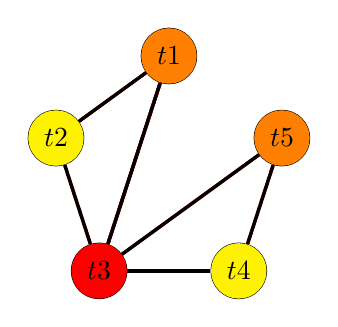
\begin{tikzpicture}[
							active/.style={red, very thick},
							default/.style={black, very thick}]
						\node[regular polygon,regular polygon sides=5,minimum size=3cm] (p) {};
						\foreach \i in {1, ..., 5} {
								\node[shape=circle,draw=black] (t\i) at (p.corner \i) {$t\i$};
							}
						\visible<4>{
							\draw[active] (t1) -- (t2);
							\draw[active] (t1) -- (t3);
							\draw[active] (t2) -- (t3);
						}
						\visible<5->{
							\draw[default] (t1) -- (t2);
							\draw[default] (t1) -- (t3);
							\draw[default] (t2) -- (t3);
						}
						\visible<5>{
							\draw[active] (t3) -- (t4);
							\draw[active] (t3) -- (t5);
							\draw[active] (t4) -- (t5);
						}
						\visible<6->{
							\draw[default] (t3) -- (t4);
							\draw[default] (t3) -- (t5);
							\draw[default] (t4) -- (t5);
						}
						\visible<6>{
							\draw[active] (t1) -- (t3);
						}
						\visible<7>{
							\draw[default] (t1) -- (t3);
						}
					
					\only<8>{
								\node[shape=circle,fill=orange] (t1) at (p.corner 1) {$t1$};
								\node[shape=circle,fill=yellow] (t2) at (p.corner 2) {$t2$};
								\node[shape=circle,fill=red] (t3) at (p.corner 3) {$t3$};
								\node[shape=circle,fill=yellow] (t4) at (p.corner 4) {$t4$};
								\node[shape=circle,fill=orange] (t5) at (p.corner 5) {$t5$};

					}

					\end{tikzpicture}
				}
			}
		\end{column}
		\begin{column}{0.5\textwidth}
						\only<-7>{
				\resizebox{0.85\textwidth}{!}{
					\begin{tikzpicture}[
							regpath/.style={blue, ultra thick},
							act_regpath/.style={red, ultra thick},
						]
						\def\numtimesteps{7}
						\def\numregisters{5}
						\foreach \i in {1, ..., \numregisters}{
								\draw (0.5, -\i) node[left] {$t\i$} -- ++(\numtimesteps, 0);
							}
						\foreach \i in {1, ..., \numtimesteps}{
								\draw[gray] (\i, -0.5) node[black, above] {$s\i$} -- ++(0, -\numregisters);
							}


						\only<2->{
							\registerpath{1}{1}{4}
							\registerpath{1}{6}{7}
							\registerpath{2}{2}{4}
							\registerpath{3}{3}{7}
							\registerpath{4}{5}{6}
							\registerpath{5}{4}{6}
							\draw[regpath] (7, -2) node[circle, draw, fill, scale=0.4] {} -- (7.5, -2);
						}

						\only<4>{
							\actregisterpath{1}{1}{4}
							\actregisterpath{2}{2}{4}
							\actregisterpath{3}{3}{7}
						}
						\only<5>{
							\actregisterpath{3}{3}{7}
							\actregisterpath{4}{5}{6}
							\actregisterpath{5}{4}{6}
						}

						\only<6>{
							\actregisterpath{1}{6}{7}
							\actregisterpath{3}{3}{7}
						}

					\end{tikzpicture}
				}}
			\only<8>{
				\begin{itemize}
					\item In Register \colorcirc{yellow} $a0$: $t2, t4$
					\item In Register \colorcirc{orange} $a1$: $t1, t5$
					\item In Register \colorcirc{red} $a2$: $t3$\\
				\end{itemize}
			}
		\end{column}
	\end{columns}
\end{frame}

\begin{frame}[c]{Single-Net Routing}{}
	\begin{columns}[t]
		\begin{column}{0.5\textwidth}
			%			\only<-7>{
			\begin{center}
				\resizebox{0.8\textwidth}{!}{
					\begin{tikzpicture}
						\tikzset{
							terminal/.style={draw, shape=circle, fill=red, inner sep=3pt},
							hanan/.style={draw, shape=circle, fill=red!30, inner sep=3pt},
							hananline/.style={color=red, dashed, very thick},
							marker/.style={draw, shape=circle, dashed, color=red, thick, inner sep=5pt},
							bboxline/.style={color=black, dashed, very thick, line cap=round},
							steinerbranch/.style={color=black, ultra thick, line cap=round}}

						\def\step{1cm}
						\def\rows{5}
						\def\cols{5}
						\def\padding{0.5cm}
						\draw[step=\step,black,thin] (0,0) grid (\cols*\step,\rows*\step);
						\draw[white] (-\padding, -\padding) rectangle (\cols*\step+\padding,\rows*\step+\padding);

						\only<4>{
							\draw[bboxline] (0,1) -- (0,3);
							\draw[bboxline] (0,3) -- (1,3);
							\draw[bboxline] (0,1) -- (1,1);
							\draw[bboxline] (1,1) -- (1,3);
						}
						\only<5->{
							\draw[steinerbranch] (0,1) -- (1,1);
							\draw[steinerbranch] (1,1) -- (1,3);
						}

						\only<7>{
							\draw[bboxline] (1,1) -- (3,1);
							\draw[bboxline] (3,1) -- (3,0);
							\draw[bboxline] (1,1) -- (1,0);
							\draw[bboxline] (1,0) -- (3,0);
						}
						\only<8->{
							\draw[steinerbranch] (1,1) -- (3,1);
							\draw[steinerbranch] (3,1) -- (3,0);
						}

						\only<10>{
							\draw[bboxline] (3,1) -- (3,2);
							\draw[bboxline] (3,2) -- (5,2);
							\draw[bboxline] (3,1) -- (5,1);
							\draw[bboxline] (5,1) -- (5,2);
						}
						\only<11->{
							\draw[steinerbranch] (3,1) -- (3,2);
							\draw[steinerbranch] (3,2) -- (5,2);
						}
						\only<13>{
							\draw[bboxline] (5,2) -- (3,2);
							\draw[bboxline] (3,2) -- (3,4);
							\draw[bboxline] (5,2) -- (5,4);
							\draw[bboxline] (5,4) -- (3,4);
						}

						\only<14, 15>{
							\draw[steinerbranch] (5,2) -- (3,2);
							\draw[steinerbranch] (3,2) -- (3,4);
						}

						\only<2>{
							% horizontal
							\draw[hananline] (0, 0) -- (5, 0);
							\draw[hananline] (0, 1) -- (5, 1);
							\draw[hananline] (0, 2) -- (5, 2);
							\draw[hananline] (0, 3) -- (5, 3);
							\draw[hananline] (0, 4) -- (5, 4);

							% vertical
							\draw[hananline] (0, 0) -- (0, 5);
							\draw[hananline] (1, 0) -- (1, 5);
							\draw[hananline] (3, 0) -- (3, 5);
							\draw[hananline] (5, 0) -- (5, 5);

							\node[hanan] at (0, 0) {};
							\node[hanan] at (0, 2) {};
							\node[hanan] at (0, 3) {};
							\node[hanan] at (0, 4) {};

							\node[hanan] at (1, 0) {};
							\node[hanan] at (1, 1) {};
							\node[hanan] at (1, 2) {};
							\node[hanan] at (1, 4) {};

							\node[hanan] at (3, 1) {};
							\node[hanan] at (3, 2) {};
							\node[hanan] at (3, 3) {};

							\node[hanan] at (5, 0) {};
							\node[hanan] at (5, 1) {};
							\node[hanan] at (5, 3) {};
							\node[hanan] at (5, 4) {};
						}

						\node[terminal] at (3, 0) {};
						\node[terminal] at (0, 1) {};
						\node[terminal] at (5, 2) {};
						\node[terminal] at (1, 3) {};
						\node[terminal] at (3, 4) {};



						\only<3,4, 5>{
							\node[marker] at (0, 1) {};
							\node[marker] at (1, 3) {};
						}

						\only<6, 7, 8>{
							\node[marker] at (3,0) {};
						}

						\only<9, 10, 11>{
							\node[marker] at (5,2) {};
						}

						\only<12, 13, 14>{
							\node[marker] at (3,4) {};
						}
					\end{tikzpicture}
				}
			\end{center}

			%	}
			%\only<8>{
			%	\begin{itemize}
			%		\item In Register \colorbox{cyan}{$a0$}: $t3$
			%		\item In Register \colorbox{yellow}{$a1$}: $t2, t4$
			%		\item In Register \colorbox{magenta}{$a2$}: $t1, t5$
			%	\end{itemize}
			%}
		\end{column}
		\begin{column}{0.5\textwidth}
			\only<1>{
				\vspace{1.5cm}
				\begin{itemize}
					\item Ziel: Verbindung von Terminalen mit kürzesten Pfaden
					\item rektilinear (geradlinig): nur horizontale/vertikale Verbindungen
				\end{itemize}

			}
			\only<2>{
				\vspace{1cm}
				\begin{itemize}
					\item Hanan-Punkte:	mögliche Steinerknoten (Abzweigungen im Steinerbaum)
					\item Schnittpunkte von Geraden durch Terminalknoten
					\item Reduziert Menge an Abzweigungspunkten, die betrachtet werden müssen
				\end{itemize}
			}

			\only<3->{
				\textbf{Konstruktion des Steinerbaums:}
				\begin{enumerate}
					\item Finde Terminale mit minimaler Manhatten-Distanz
					      \only<4->{
					\item Konstruiere die kürzesten Verbindungen (bounding box)}
					      \only<5->{
					\item Wähle die Verbindung, welche den geringsten Abstand zu einem der anderen Terminalknoten hat
					      }
					      \only<6->{
					\item	Finde Terminale mit minimaler Manhatten-Distanz zur konstruierten Verbindung und fahre mit Schritt 2 fort
					      }
				\end{enumerate}
			}


		\end{column}
	\end{columns}

\end{frame}



\begin{frame}[c]{}{}
	\begin{center}
		\LARGE Fragen?\\
		\vspace{\baselineskip}
		\normalsize Die Slides zur Registerallokation wurden von \href{https://home.cit.tum.de/~hbj/}{Bjarne Hansen} übernommen
	\end{center}
\end{frame}

\begin{frame}[c]{Artemis-Hausaufgaben}{}
	\begin{itemize}
		\item \enquote{H13 -- Verifikation mit SAT} bis 02.02.2025 23:59 Uhr
		\item Finden der KNFs für zwei Miter-Schaltungen
		\item letzte Hausaufgabe -- Notenbonus ab 80\% (exklusive Bonuspunkte)
	\end{itemize}
\end{frame}

\begin{frame}[c, fragile]{Links}{}
	\begin{itemize}
		\item Zulip: \href{https://zulip.in.tum.de/#narrow/stream/2661-ERA-Tutorium---Do-1600-1}{\enquote{ERA Tutorium - Do-1600-1}}
		      bzw. \href{https://zulip.in.tum.de/#narrow/stream/2675-ERA-Tutorium---Fr-1500-2 }{\enquote{ERA Tutorium - Fr-1500-2}}
		\item \href{https://www.moodle.tum.de/course/view.php?id=100633}{ERA-Moodle-Kurs}
		\item \href{https://artemis.in.tum.de/courses/401}{ERA-Artemis-Kurs}
	\end{itemize}
\end{frame}

\maketitle

\end{document}
